
\chapter{Background}
\section{Entropy, relative entropy and mutual information}
We first discuss specific definitions from information theory. These concepts will be relevant to understand contrastive predictive coding, which we discuss in a following section. The formal definitions are obtained from the book "Elements of Information Theory" \cite{coverELEMENTSINFORMATIONTHEORY}. The equations that contain a log function are assumed to be under base two.
\subsection{Shannon's Entropy}
Entropy measures the average amount of information required to describe a random variable \cite{coverELEMENTSINFORMATIONTHEORY}. The entropy H(X) of a discrete random variable $X$, is formally defined in equation \ref{eq:entropy} shown below. 

\begin{equation}
	H(X) = -\sum_{x\in\mathcal{X}} p(x) \log p(x)  \label{eq:entropy}
\end{equation}

The alphabet $\mathcal{X}$ represents the set of events the random variable X can take, formerly known as the \textit{sample space}. Additionally, $p: \mathcal{X} \rightarrow [0, 1]$ denotes the probability density function of $X$. Hence, given an event $ x \in \mathcal{X}, p(x) $ corresponds to the probability of event x occurring.

%[general explanation]
Assume a random variable $X$ with possible events $x_1$, $x_2$. Intuitively, when $p(x_1)$ is low, the surprise when the event $x_1$ occurs will be high. The surprise for one event is denoted in equation \ref{eq:surprise}. 

\begin{equation}
	-p(x) \log p(x) \label{eq:surprise}
\end{equation}

Hence, entropy can also be considered as the sum of “surprise” over each event \cite{datasciencecoursesAliGhodsiLec2017}. 
%[algebraic explanation]
To understand why equation \ref{eq:surprise} does indeed correspond to a measure of surprise, consider an event $x \in \mathcal{X}$ with $p(x) = 1$. Note that $\log p(x) = 0$, and thus the surprise is zero. Meanwhile, if p(x) approaches $0$, $\log p(x)$ goes to $- \inf$. And hence, by the negation sign in formula \ref{eq:entropy} the surprise is large.


\begin{figure}[h]
	\centering
	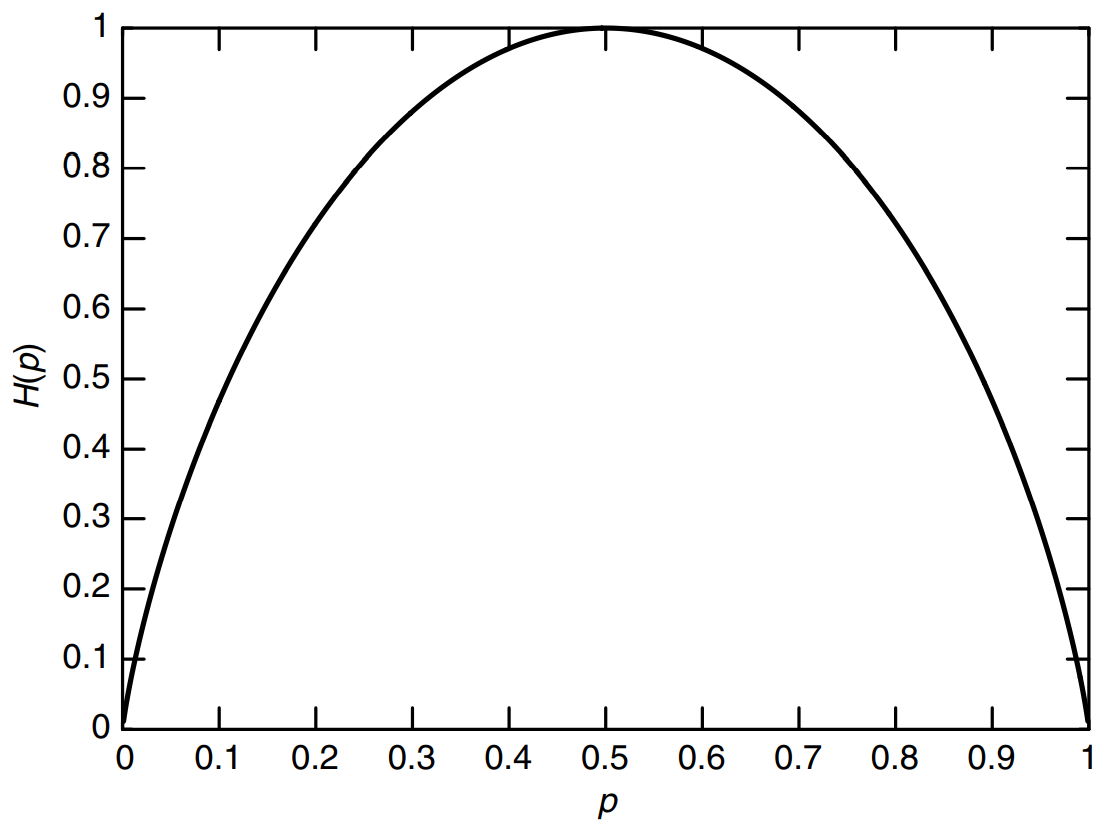
\includegraphics[width=0.4\linewidth]{screenshot005}
	\caption{$H(p)$ vs $p$ (originates from "Elements of Information Theory", page 16)}
	\label{fig:EntropyvsP}
\end{figure}



%[book: p16: note should rename figure to axes to ” H(x) vs …”]
Figure \ref{fig:EntropyvsP} displays when entropy reaches its maximum for the case of a random variable with 2 outcomes. We can see that the entropy, and thus, the information is largest when the probability of the two outcomes is equal to each other, namely $p(x_1)=p(x_2)=0.5$. Note that for a random variable $X$ with more than two events, $H(X)$ can be larger than one.

\subsection{Relative entropy and mutual information}
Relative entropy, also known as the Kullback Leibler (KL) divergence, is defined in equation \ref{eq:kl}, where $p$ and $q$ denote a probability density function over the same sample space $\mathcal{X}$ \cite{coverELEMENTSINFORMATIONTHEORY}. The KL divergence quantifies the “divergence” or "distance" between the two distributions. Note that $D(p||q)$ does not necessarily correspond to $D(q||p)$ and thus the metric is not symmetrical.

\begin{equation}
	\kl{q}{p} = \sum_{x\in\mathcal{X}}p(x) \log \frac{p(x)}{q(x)} \label{eq:kl}
\end{equation}



% was rephrased by chat gpt
The mutual information (MI) between two random variables $X$ and $Y$ can be computed as the KL divergence between their joint probability distribution, $p_{X,Y}(x,y)$, and the product of their marginal probability distributions, $p_X(x)$ and $p_Y(y)$, which is denoted as $p_X(x)p_Y(y)$ \cite{coverELEMENTSINFORMATIONTHEORY}. The equation for mutual information then becomes:

\begin{equation}
	I(X; Y) =  \kl{p_{X, Y}(x, y)}{p_X(x) p_Y(y)}
\end{equation}

As described by Cover and Thomas in their book "Elements of Information Theory" \cite{coverELEMENTSINFORMATIONTHEORY}, I(X; Y) quantifies the amount of information $Y$ describes about $X$. A alternative definition for $I(X;Y)$ is illustrated in \ref{eq:MI_reduce}. The equation provides us with an intuitive meaning for $I(X;Y)$, corresponding to the surprise caused by $X$, which is reduced by the knowledge of $Y$. In a following section, we discuss how these concepts from information theory are applied in representation learning, by maximising the mutual information between latent representations.

\begin{equation}
	I(X;Y)= H(X) - H(X|Y) \label{eq:MI_reduce}
\end{equation}



\section{Supervised neural networks}

% COMMENT CHAT GPT: WHAT IS THE PURPOSE OF THIS SECTION?
%Clarify the purpose of the section: The section starts by stating that it will discuss traditional supervised learning approaches, but it's not entirely clear what the purpose of the section is. Are you providing an introduction to supervised learning for readers who may be unfamiliar with it? Or are you focusing on the specifics of how supervised learning is implemented with ANNs?

We shall now discuss traditional supervised learning approaches, as these will lay the groundwork for the representation learning approaches discussed in the following section. 

Typical supervised machine learning problems consider the problem where given a training set of tuples ($x_i$, $y_i$), a mapping function $f: \mathcal{X} \rightarrow \mathcal{Y}$ must be learned, where $x_i \in \mathcal{X}$ corresponds to the input sample and $y_i \in \mathcal{Y}$ the label. A good $f$ will then also generalise well to unseen $x_i \in \mathcal{X}$, which were not part of the training set.

Artificial Neural Networks (ANNs) in particular, tackle this problem by defining $f$ as a fixed set of parameters consisting of a series of layers. During inference, at each layer $l$ a transformation matrix $W^l$ is applied to the output vector from the previous layer $a^{l-1}$. This is shown in the equation below.

$$ z^l = W^l a^{l-1} $$

Secondly, a non-linear function $\sigma: R^d \rightarrow R^d$ is applied to $z^{l}$, as shown in equation \ref{eq:nonlinearity}. The resulting vector $a^l$ may then again be the input for a following layer.

\begin{equation}
	a^l = \sigma(z^{l})	\label{eq:nonlinearity}
\end{equation}

Hence, during inference, the input vector $x$ is propagated through each layer, resulting in a final output $\hat{y}^L$. The equation for the forward pass of a neural network with $L$ layers is described in equation \ref{eq:forward_pass}. 

\begin{equation}
	f_{W^1 \dots W^L}(x) = \hat{y}^L = \sigma(… \sigma( \sigma( x^T W^1 )^T) W^2 …)^T W^L \label{eq:forward_pass}
\end{equation}

% [cost function, gradient descent, backpropagation]
During training the ANN's parameters $W^1$ \dots $W^L$, are optimised according to the learning problem. The viability of the parameters is quantified by the loss function $\mathcal{L}$ over a batch of $n$ training samples, as shown in equation \ref{eq:generic_loss}. $y_i$ corresponds to the ground truth label of the single data sample $x_i$, $e(y_i, \hat{y}_i)$ the error between a ground truth $y_i$ and the estimation $\hat{y}_i$ of a single sample. The error function $e$ can be replaced depending on the task, for instance by mean squared error for regression or cross entropy for classification problems.

\begin{equation}
	\mathcal{L}(W) = \frac{1}{n}\sum_{i=1}^n e(y_i, f_{W}(x_i)) \label{eq:generic_loss}
\end{equation}

The parameters can be optimised by minimising the loss function $\mathcal{L}$ defined above. This can be done algebraically, however, it becomes difficult when the dimension of the input features is large. Gradient descent is used to find an "appropriate" minimum of the cost function, by iteratively adjusting the parameters $W^1$ \dots $W^L$ via the following learning rule.

\begin{equation}
	W^l_{ij} \leftarrow W^l_{ij} - \alpha \frac{\partial \mathcal{L}}{\partial W^l_{ij}}
\end{equation}

Although gradient descent can be successfully applied for finding local minima, neural networks may still contain many parameters which each must be optimised. This is typically resolved by applying the backpropagation algorithm in combination with gradient descent, such that fewer partial derives must be calculated, resulting in more efficient optimisation.


% review from chat gpt:
%Lastly, it would be useful to provide some discussion of the limitations of supervised learning approaches, beyond the issue of requiring large amounts of labelled data. For example, it would be worth noting that these techniques can be prone to overfitting, and that they may not be well-suited to tasks where the relationship between inputs and outputs is highly complex or non-linear.


% limitations of supervised learning approaches and towards representation learning
% TODO: this paragraph should be better written
Although supervised learning though ANNs is considered successful, their performance is heavily dependent on the choice of the data representation \cite{bengioRepresentationLearningReview2013}, on which they are applied. For complex representations, a more complex architecture may be required, which requires more data to prevent overfitting. When labelled data is scarce, these models may result in seemingly well performance on the training set, but bad generalisation to data outside the training set. As a consequence, a lot of time in the machine learning pipeline is invested in transforming data into better latent representations. Good latent representations tend to disentangle the data into meaningful features, such that data can be more easily be separable into classes. In the following section we discuss how part of the labour of finding good representations can be relieved with unsupervised learning approaches, which may learn to find good latent representations. These representations could then be used as the input for supervised predictors.




\section{Representation learning through reconstruction error}
%[what is repr learning]
One of the challenges in supervised learning is the constant need of large amounts of labelled data. Hence, when a labelled dataset is small, we would like to leverage a larger unlabelled dataset as basis for learning. By doing so, a mapping can be learned from the raw input data to a representation which makes downstream tasks easier. This process of learning representations from data is commonly referred to as representation learning \cite{le-khacContrastiveRepresentationLearning2020}. Supervised learning algorithms can then learn directly from these disentangled latent representations with fewer labelled data.

In the following two sections we discuss two paradigms of representation learning with ANNs. The first paradigm is learning representations by minimising a reconstruction error. The second learns its representations by contrasting them against noise. These two paradigms will lay the basis for our own contributions in section three.

\subsection{Autoencoders}
%auto encoder: good at capturing complex, high-dimensional features of the input data
%\textbf{WHY: More interpretable latent representations through Gaussian distributions.}
Autoencoders were introduced in 1986 by D. Rumelhart et al. \cite{rumelhartLearningInternalRepresentations1988} as a means to learn compressed representations \cite{bankAutoencoders2021}. This is achieved through a neural network architecture consisting of two blocks. The first block is the encoder $E$ and receives input data which it encodes into a lower dimensional representation. The second block, called the decoder $D$, receives as input the latent representation and is tasked to reconstruct the original input. The two blocks are simultaneously optimised by \textit{minimising the reconstruction error} shown in the following equation:

\begin{equation}
	\mathcal{L} = \sum_{i = 1}^N l(\vecti{x}, D(E(\vecti{x})))
\end{equation}

where $l$ refers to the error for a single data point, for instance the $l_2$-norm and $N$ the number data points. An example autoencoder architecture is depicted in figure \ref{fig:autoencoder}. $\vect{x} \in \mathcal{D}$ corresponds to an input vector which is encoded into latent representation $\vect{z}$. The decoding of $\vect{z}$ corresponds to $\tildex = D(E(\vect{x}))$. The dimension of $\vect{z}$ is typically bottlenecked to be smaller than the original dimension of $\vect{x}$. This results in the encoder having to define encodings that are as "informative" as possible to reconstruct the original data \cite{bankAutoencoders2021}. $\vect{z}$ may then for instance be used for downstream tasks such as classification or clustering.

\begin{figure}
	\centering
	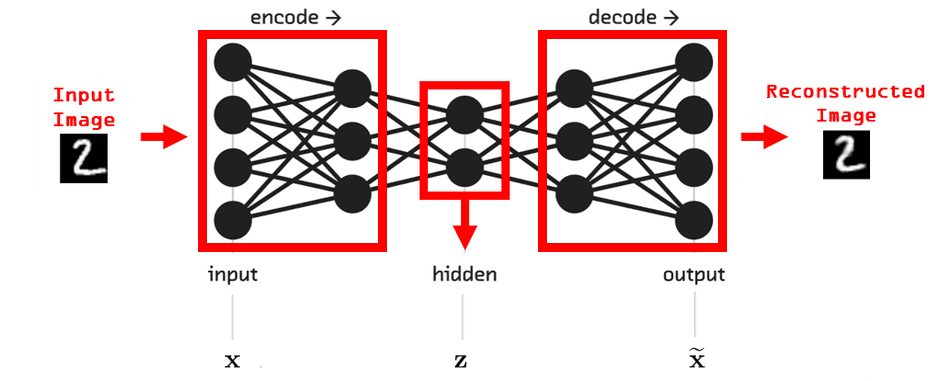
\includegraphics[width=0.7\linewidth]{autoencoder}
	\caption{Autoencoder neural network architecture adapted from \cite{karagiannakosHowGenerateImages2018}.}
	\label{fig:autoencoder}
\end{figure}


%motivations for VAE
While capable of learning compressed representations, autoencoders do not pose any restrictions on the latent space they define (the space of latent representations). As a result, the representations may be meaningful to computers, but non-interpretable to humans. For instance, given the left image depicted in figure \ref{fig:latent_space_2d} which depicts an autoencoder's two dimensional latent space, it is very difficult to know what the resulting images would be when interpolating between the latent representations of 0 (red) and 1 (blue). Answering this question becomes even more infeasible for higher dimensional latent vectors.

\begin{figure}
	\centering
	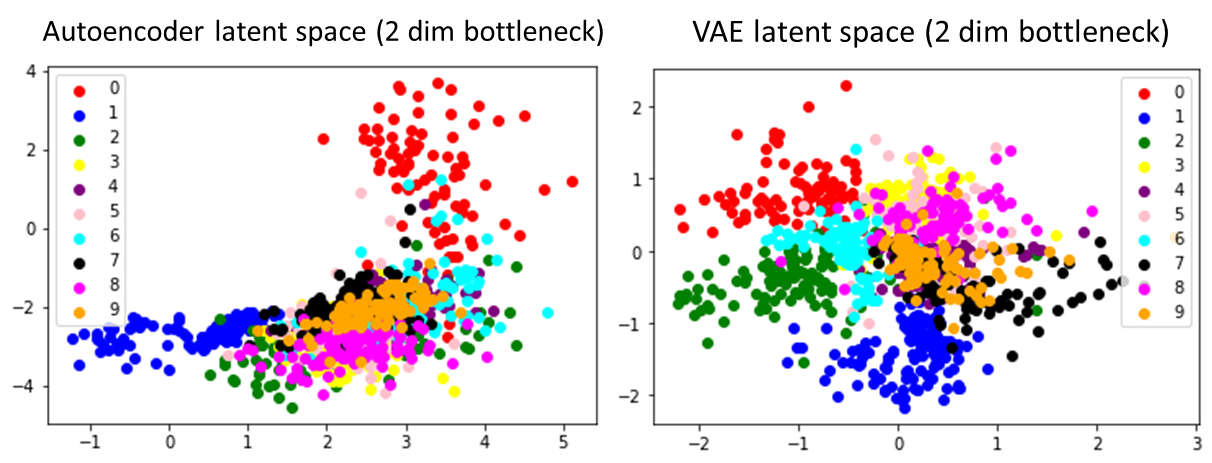
\includegraphics[width=0.7\linewidth]{screenshot021}
	\caption{ Both images represent a the two-dimensional latent space, learned from the MNIST dataset \cite{PapersCodeMNIST}. This is a dataset consisting of images of handwritten numbers between 0 and 9. Each image is associated to a class label, referring to the number. The left image consists of the space learned from a classical autoencoder, the right of a variational autoencoder (VAE). Both autoencoders have not received any explicit information of the labels of the dataset, yet learned to define representations which equal numbers are closer to each other. The VAE's latent space, depicted in the right image, is optimised to be standard normally distributed. The latent vectors $\vect{z}$ are distributed according to the two-dimensional normal distribution $\sample{\vect{z}}{\standardnormal}$, where $\bm{\mu}$ is the two dimensional zero vector. $\identitymtx$ is the $2 \times 2$ covariance matrix with ones on the diagonal and zeroes elsewhere.}
	\label{fig:latent_space_2d}
\end{figure}

\subsection{Variational autoencoders}
% notes: 
%1) discuss why, (latent space gaussian)
%2) architecture predicting values
%3) explicit elbo (where q is optimised to be Gaussian) and give intuitions how it squishes all data points together
%4) can be used for latent space, or also 
%4) link with maximising likelihood -> p(x) and how minimises kl divergence between approx and kl divergence

Similar to traditional autoencoders, variational autoencoders (VAE) learn representations that contain the important information that is necessary to reconstruct the data, \textit{however}, an additional constraint is applied to the latent space \cite{doerschTutorialVariationalAutoencoders2021, davidfosterVariationalAutoencoders2023, kingmaAutoEncodingVariationalBayes2022, kingmaIntroductionVariationalAutoencoders2019, cinelliVariationalMethodsMachine2021}. The data points from the latent space are defined in such a way that they conform to a certain distribution, typically, the standard normal distribution $\standardnormal$ \cite{davidfosterVariationalAutoencoders2023}. % ref book oreiley
%The standard normal distribution is a Gaussian distribution (a symmetric distribution characterised by a bell shape), with with a mean of zero and a standard deviation of one \cite{bhandariStandardNormalDistribution2020}. 
This behaviour can be observed in the right plot of figure \ref{fig:latent_space_2d}. Since the latent representations conform a two-dimensional standard normal distribution $\standardnormal$, the data samples are more likely to be near the center at (0, 0).

% TODO: explain about gaps, etc
% i said z's are closer to (0, 0). why do we care? -> similar points are still clustered together, however, there will not be any gaps in the latent space. can thus interpolate between latent representations to find meaningful datapoints.

%o reiley:
%\textit{"A multivariate standard normal distribution is a multivariate distribution with zero valued mean vector and identity covariance matrix."} - 
%%https://learning.oreilly.com/library/view/generative-deep-learning/9781098134174/ch03.html#normal_distribution
%
%\textit{Previously, we saw how there was no requirement for the latent space to be continuous—even if the point (–2, 2) decodes to a well-formed image of a sandal, there was no requirement for (–2.1, 2.1) to look similar. Now, since we are sampling a random point from an area around $z_mean$, the decoder must ensure that all points in the same neighborhood produce very similar images when decoded, so that the reconstruction loss remains small. This is a very nice property that ensures that even when we choose a point in the latent space that has never been seen by the decoder, it is likely to decode to an image that is well formed.} - o reiliy
%





%\textbf{How: predict distributions}

\subsubsection{Simulating distributions through neural networks}
In variational autoencoders the latent representations of a data point $\vecti{x}$ does not simply consist of a fixed deterministic vector $\vecti{z}$, as was the case in the traditional autoencoder. Instead, given $\vecti{x}$, its latent representation corresponds the following distribution $\qphizx$.
A concrete vector $\vecti{z}$ can be obtained taking a sample $\sample{\vecti{z}}{\qphizx}$. As result a single $\vecti{x}$ will correspond to multiple latent vectors $\vecti{z}$. The latent representation $\qphizx$ is modelled as $\normal$. This means that all the required information to model $\qphizx$ is a mean vector $\mui$ and a covariance matrix $\diagsigmai$. Thus, given $\vecti{x}$, a deterministic neural network can simulate $\diagsigmai$ by predicting two vectors, namely, $\mui$ and $\sigmai$. The latent vectors $\vecti{z}$ can then be obtained by randomly sampling from the distribution. And thus, multiple $z^{(i)}$'s may correspond to a single $\vecti{x}$. This method is depicted in figure \ref{fig:vae-repr}. Finally, a sample $\vecti{z}$ can be obtained as follows:

\begin{equation}
\vecti{z} = \mui + \sigmai \odot \epiloni
\end{equation}

where $\epiloni$ corresponds to a sampled value $\samplestandardnormal{\epiloni}$ and $\odot$ is element-wise multiplication. Computing $\vecti{z}$ through $\epiloni$, rather than directly sampling from $\sample{\vecti{z}}{\normal}$ is referred to as the parametrisation trick and allows for gradients to freely backpropagate through the layer \cite{davidfosterVariationalAutoencoders2023}.


% TODO: die sigma(i) moet ^2 zijn!!
\begin{figure}
	\centering
	\includegraphics[width=0.6\linewidth]{"vae repr"}
	\caption{High level view of a variational autoencoder, depicting how a data point $\vecti{x}$ is encoded into a latent distribution and reconstructed as $\tildexi$. Both blocks depict a neural network. The upper block is the encoder and the lower block the decoder. The upper block receives a data points $\vect{x}$ and produces the parameters of $\qphizx$. Since we choose to model $\qphizx$ as a Gaussian with independent components, the covariance matrix $\covariancemtx$ is zero everywhere except for the diagonal. This way the diagonal values, representing the standard deviations, can be represented via a single vector $\sigmai$. The vectors $\mui$ and $\sigmai$ are $\mu(\vecti{x})$ and $\sigma(\vecti{x})$, respectively. These are the output of the encoder block and form the parameters for $\qphizx$. A single neural network with parameter weights $\phi$ is used to simulate $\qphizx$ for every $\vecti{x} \in \mathcal{D} $. This strategy of sharing $\phi$ across data points is refered to as "amortised variational inference" \cite{kingmaIntroductionVariationalAutoencoders2019}.}
	\label{fig:vae-repr}
\end{figure}

%$$\vecti{x} \in \mathcal{D} $$
%$$\vect{z}$$
%$$\mu(\vect{z})$$
%$$\sigma(\vect{z})$$
%
%$$\mu(\vecti{x})$$
%$$\sigma(\vecti{x})$$
%
%
%$$\sample{\vect{z}}{\normal}$$
%
%
%$$ \qphizx $$
%$$ \pthetaxz $$
%
%$$ \widetilde{\mathbf{x}} ^ {(i)} $$

\subsubsection{The learning objective}

So far we have discussed how predictions of a neural network can emulate predicting a distribution $\qphizx$, by predicting the distribution's parameters $\mui$ and $\sigmai$. However, no constraints have been set on the quality of the distributions. We will discuss this now. The representations are optimised to minimise two measurements: one, the reconstruction error, and secondly, the distance from the latent distributions to $\standardnormal$.

The loss function to be optimised for a single data point $\vecti{x}$ is shown in the equation below.

\begin{equation}
	\mathcal{L}_{\theta, \phi} (\vecti{x}) = \elboexplicit \label{eq:elbo_explicit_intial}
\end{equation} % src: ref to slides ugent

% 1) reconstruction error
Although the equation may seem daunting at first, we will decompose its components. The loss function is made up of two terms, the left term corresponds to the reconstruction error, while the second term poses constraints on the latent space. Let us focus on the reconstruction term first.

$$
\reconstr
$$

The distribution $\pthetaxz$ is a distribution over $\vecti{x}$ where $\vect{z}$ is instantiated. What comes out are thus probabilities. Notice $\vect{z}$ is sampled from the Gaussian distribution $\sample{z}{\qphizx}$. So the $\vect{z}$'s close to the mean $\mu(\vecti{x}) = \mui$ are more likely to be sampled than those further away. So for these $\vect{z}$'s, we'd like the probability of corresponding to the actual $\vecti{x}$ to be high. Finally, by adding a negative sign in front, maximising this probability is equivalent to minimising the negative probability \cite{pinheirocinelliVariationalAutoencoder2021}. % TODO: FOR SOME REASON REFERENCE NOT FOUND 
%Additionally, minimising this term is equivalent to maximising the likelihood of the reconstructed sample $\vecti{x}$. 
In practice this term is approximated through mini-batches with the mean squared error. %todo: look into max like estim, as there hopefully i can find a meaningful defintion for "maximising..."


Optimising the second term of equation \ref{eq:elbo_explicit_intial} poses the constraints on the latent distributions $\qphizx$. Again, this metric should be minimised. As we discussed in the chapter on Entropy, the KL divergence can be considered as a (non-symmetric) distance measure between two distributions. Hence, this value is small when the two distributions are similar. As we discussed earlier $\pz$ is often replaced by $\standardnormal$ as shown below. Minimising this equation will result in moving each distribution $\qphizx$, corresponding to a value $\vecti{x}$, close to $\standardnormal$.

$$
\latentspaceconstraintstandardgaussian
$$


One can algebraically prove, that optimising this equation is equivalent to optimising the following equation \cite{kingmaAutoEncodingVariationalBayes2022}: 

\begin{equation}	
	\kl{\normal}{\standardnormal} = \latentspaceconstraintclosedform
\end{equation}

where $\sigma_k^{(i)}$ and $\mu_k^{(i)}$ correspond to the components of the predicted vectors $\sigmai$ and $\mui$, respectively.


% 2) kl divergence

\subsubsection{[TODO] Relation with variational inference / derivation of ELBO loss}

%A mapping function $f_W(x) = y$ can be predict distributions by predicting the parameters of the the distribution (mu, sigma for Gaussian distributions).
%
%Rather than directly learning parameters $\phi$ that map a data point $\vecti{x}$ to latent distribution $p(\vect{z} \mid \mathbf{x}^{(i)})$, an \textit{approximate distribution} $\qzx$ is learned that approximates $p(\vect{z} \mid \vecti{x})$. Through gradient descent parameters for $\phi$ can be achieved, by minimising the KL divergence between the two distributions. $\condq{\vect{z}}{\vecti{x}}$ will is expressed as Gaussian distribution.
%
%
%\begin{equation}
%	\kl{\qprobzx}{\probzx} \label{eq:kl_q_p}
%\end{equation}
%
%Yet, the idea is nice, optimising $\qprobzx$ to approximate $\probzx$ sounds nice, it is only possible when $\probzx$ is known, which it is not. If it was, there was no need to approximate it.
%
%Equation \ref{eq:kl_q_p} is thus intractable to compute, yet the following is true:
%
%\begin{equation}
%	\begin{aligned}
%		\kl{\qprobzx}{\probzx} & = \expectedsamplezq \left[ \log \frac{\qzx}{\pzx} \right] \\
%		& = ... (todo) \\
%		& = - \left( \elbo \right) + \logevidence
%	\end{aligned}
%\end{equation}
%
%By replacing the terms, we obtain the following equation:
%
%\begin{equation}
%	\begin{aligned}
%		\logevidence & = 
%		\klapproxposterior + \elbo \\
%		& = \klapproxposterior  + \lelbo
%	\end{aligned}
%\end{equation}
%
%We can observe that the KL divergence between the true and approximate posteriors, $p$ and $q$ respectively, is bounded by $\logevidence$. Hence, although $\pzx$ is unknown, maximising $\lelbo$ results in minimising the KL divergence. Also notice that $\kl{\qprobzx}{\probzx} >= 0$, and thus the maximum value for $\lelbo$ results in a KL divergence between the posteriors of zero. It thus suffices to maximise $\lelbo$, or equivalently minimise $-\lelbo$. The loss for a single data point $\vecti{x}$ then becomes

%TODO \textbf{todo: in paper variational bayes, they refer to p(x) as p theta, but in slides ugent not?}. \textbf{todo: why cant p(x) be very big then? probably has something to do with jensens inequality.}




\begin{equation}
	\begin{aligned}
		- \lelbo & = - \elbo \\  
		& = \elboexplicit \label{eq:elboexplicit} \\
	\end{aligned}	
\end{equation} % src: ref to slides ugent

Where the first term is reconstruction error and second is regularisation. Hence minimising the KL divergence between the two posteriors is equivalent to minimising the divergence between the approximate posterior $\qzx$ and the \textbf{marginal or prior?} $\pz$.

$p(z)$ in the equation is usually chosen to be the standard normal distribution $\mathcal{N}(0, I)$, such that a closed form solution exists. As such, when $p(z)$ corresponds to the standard normal, and $\qzx$ is a multidimensional Gaussian with mean vector $\mui$ and covariance matrix with independent dimensions, such that the diagonal corresponds of a vector standard devisations $\sigmai$, then the KL divergence has the following closed form:

\begin{equation}	
	\kl{\normal}{\standardnormal} = \latentspaceconstraintclosedform
\end{equation}

For the equation above, gradients can easily be back propagated through machine learning libraries such as Tensor Flow. We still require a method for computing the gradient of the first term in $\lelbo$. % todo: gradient van linker kan door sampling en mini batch.











%Recent Advances in Autoencoder-Based:
%Representation Learning https://arxiv.org/pdf/1812.05069.pdf
%they speak about disentanglement of vae and indepndent features

%Understanding disentangling in β-VAE
%https://arxiv.org/pdf/1804.03599.pdf
%"β-VAE aligns latent dimensions with components that make different contributions to reconstruction"
%Our key hypothesis is that β-VAE finds latent components which make different contributions to the log-likelihood term of the cost function (Eq. 5). These latent components tend to correspond to features in the data that are intuitively qualitatively different, and therefore may align with the generative factors in the data.











%- \subsubsection{reparametrisation trick}
%o reiley:
%\textit{THE REPARAMETERIZATION TRICK
%	Rather than sample directly from a normal distribution with parameters $z_mean$ and $z_log_var$, we instead sample epsilon from a standard normal and then manually adjust the sample to have the correct mean and variance.}
%\textit{This is known as the reparameterization trick and is important as it means gradients can backpropagate freely through the layer. By keeping all of the randomness of the layer contained within the variable epsilon, the partial derivative of the layer output with respect to its input can be shown to be deterministic (i.e. independent of the random epsilon), which is essential for backpropagation through the layer to be possible.}

%\subsubsection{the loss function - from oreiley}
%The Loss Function
%Previously, our loss function only consisted of the reconstruction loss between images and their attempted copy after being passed through the encoder and decoder. The reconstruction loss also appears in a variational autoencoder, but we require one extra component: the Kullback–Leibler (KL) divergence term.
%
%KL divergence is a way of measuring how much one probability distribution differs from another. In a VAE, we want to measure how much our normal distribution with parameters z_mean and z_log_var differs from a standard normal distribution. In this special case, it can be shown that the KL divergence has the following closed form:
%
%kl_loss = -0.5 * sum(1 + z_log_var - z_mean ^ 2 - exp(z_log_var))
%or in mathematical notation:
%
%The sum is taken over all the dimensions in the latent space. kl_loss is minimized to 0 when z_mean = 0 and z_log_var = 0 for all dimensions. As these two terms start to differ from 0, kl_loss increases.
%
%In summary, the KL divergence term penalizes the network for encoding observations to z_mean and z_log_var variables that differ significantly from the parameters of a standard normal distribution, namely z_mean = 0 and z_log_var = 0.
%
%Why does this addition to the loss function help?
%
%Firstly, we now have a well-defined distribution that we can use for choosing points in the latent space—the standard normal distribution. Secondly, since this term tries to force all encoded distributions toward the standard normal distribution, there is less chance that large gaps will form between point clusters. Instead, the encoder will try to use the space around the origin symmetrically and efficiently.
%
%In the original VAE paper, the loss function for a VAE was simply the addition of the reconstruction loss and the KL divergence loss term. A variant on this (the 
%-VAE) includes a factor that weights the KL divergence to ensure that it is well balanced with the reconstruction loss. If we weight the reconstruction loss too heavily, the KL loss will not have the desired regulatory effect and we will see the same problems that we experienced with the plain autoencoder. If the KL divergence term is weighted too heavily, the KL divergence loss will dominate and the reconstructed images will be poor. This weighting term is one of the parameters to tune when you’re training your VAE.



%\subsubsection{Disentangled latents + posterior collapse}


\section{Representation learning through Noise-contrastive estimation}




% FEEDBACK: MORE EXPLICITLY STATE MAIN IDEA OF REPR LEARNING AND HOW CPC FITS INTO THIS FRAMEWORK
\subsection{Contrastive predictive coding}


%\textbf{[What: CPC: repr for sequences]} \\
	In what follows next, we discuss Contrastive Predictive Coding (CPC), a representation learning approach that we use as the basis for our own experiment in the following chapter.
	% TODO: cpc differs from autoencoders in two key ways: reconstruct + time series data
	CPC is an unsupervised learning approach, again with the objective of learning (lower dimensional) representations from high dimensional data \cite{oordRepresentationLearningContrastive2019}. While the objective is thus the same as for the autoencoders discussed in the previous section, CPC achieves its representations entirely differently. An autoencoder's objective is to define a compressed representation from which the original data can be recovered. However, when working with sequential data, compressing patches of the sequence without considering the relation with nearby patches, will result in lost information as the context between patches is not encoded into the representation. % todo: is based on blog, but i cant really refer.. https://www.lesswrong.com/posts/XE6LD2c9NtB7gMdEm/an-92-learning-good-representations-with-contrastive. I should however give an example.


\begin{figure}[h] % cpc overview
	\centering
	\includegraphics[width=0.7\linewidth]{"cpc overview"}
	\caption{Overview of Contrastive Predictive Coding, originates from \cite{oordRepresentationLearningContrastive2019}}
	\label{fig:cpc-overview}
\end{figure}

%\textbf{[maintain information between patches by predicting the future based on the past? + architec fig + var names]} \\
	% todo
	CPC deals with these context issues by maximising the shared information between the extracted representations of temporally nearby patches \cite{lowePuttingEndEndtoEnd2020}. We will discuss this concept in more detail in a following section. For now, we would like to draw the readers attention to figure \ref{fig:cpc-overview}. The figure depicts a high level view of how this idea is achieved by producing two latent latent representations $\vect{z}_i$ and $\vect{c}_i$. An audio sequence of undefined length is split up into patches $\x_1 \dots \x_n$ where each $\x_i$ is a vector of fixed length, containing for instance 10ms of speech audio. Each patch $\x_i$ is encoded into latent representation $\zt$, defined as follows:
	
	$$
	\zt = g_{enc}(\xt) .
	$$
	
	$g_{enc}( \cdot )$ is for instance a convolutional fully connected ANN. The latent representations $\z_1..\z_n$ are obtained independently from each other and do not yet contain any information on an historic context. This historic context is achieved through $g_{ar}( \cdot )$, an auto-regressor, which encodes all previous $\z_1 \dots \zt$ into a single representation $\ct$:
	
	$$
	\ct = g_{ar}(\z_1 \dots \zt)
	$$
	
	Either $\zt$ or $\ct$ could be used as latent representation for downstream tasks. Oord et al. suggest to use $\ct$ for tasks where context about the past is useful, for instance speech recognition, and $\zt$ when historic context is not useful \cite{oordRepresentationLearningContrastive2019}. As shown in figure \ref{fig:cpc-overview}, the encodings from sequential data of undefined length, may correspond a series of latent representations $\vect{c}_1, \vect{c}_2, \dots $ or $\z_1, \z_2, \dots $. In the case of downstream tasks which require a single representation vector, Oord et al. propose to pool the sequence of vector representations into a single vector.
	

\subsubsection{Slowly varying features}
%\textbf{[assume slow features. + why maxim mutual info? between past and future]}\\
	The temporally nearby patches $\z_{t+1}$ and $\ct$ are optimised to preserve shared information, while discarding differences. Before we discuss how to obtain such representations, we first motivate why defining representations in this fashion makes sense.
	
	Consider we would like to define useful representations for sequential data such as speech signals. Then it not unlikely to believe that the conveyed information at time step $t$ and $t+k$ contains some redundant information, such as pitch, frequency, tone, etc. \cite{raoUnderstandingGradientIsolatedLearning2020}. Meanwhile, large changes of the signal in a small time window, may be the result of noise. Sequential data which poses these slowly varying features, are commonly referred to as "slow-features" \cite{zhangSlowFeatureAnalysis2012}. CPC leverages these slowly varying features, by encoding the underlying shared information between different patches, while at the same time discarding low-level information and noise that is more local \cite{oordRepresentationLearningContrastive2019}.


\subsubsection{The learning objective}
%\textbf{[discriminate pos from neg samples + formal MI]}\\
	% the latent representations are optimised through a similarity function f. It will turn on that optimising the similarity between two representations is equivalent to maximising their mutual information.
	
	
	CPC will learn to preserve information between temporally nearby representations, by solving another task. In particular, CPC learns to discriminate subsequent \textit{positive} samples $\ztk$ from \textit{negative} random samples $\zj$. This is achieved through a similarity function $f_k(\cdot)$, which scores the similarity between two latent representations \cite{lowePuttingEndEndtoEnd2020}. It is defined as a log bilinear model as follows:
	\begin{equation} % f_k
		\fkdefinition \label{eq:fk}
	\end{equation}
	where $W_k$ is a weight matrix which is learned. $f_k( \zj , \ct )$ thus quantifies how likely the context $\ct$ corresponds to a random vector $\zj$. Due to the slowly varying data assumption, a good representation for successive representations $\ztk$ and $\ct$ is one where $f_k( \ztone, \ctone)$ is high and $f_k( \zj, \ct)$ is small for random $\zj$. Or equivalently, maximising the shared information between temporally nearby patches, while discarding the temporal noise results in large values $f_k( \ztone, \ctone)$.
	%Had er miss ergens bij gekund: Finding the correct $\ztone$ in a batch of random $zjs$, given $\ct$ is thus equivalent to "predicting the future given the past" (is related to predictive coding).
	
	%	CPC learns to discriminate subsequent 'positive' samples $x_{t+1}$ from 'negative' random samples $\x_j$, hence the name “contrastive noise estimation”. CPC exploits this so called ‘slow-features’ property, by encoding the common information between nearby parts of the signal, while also ignoring the noise which is more local. It will turn out that maximising this shared information, corresponds the notion of mutual information, we discussed earlier. We discuss this more in more detail in a following subsection.
	%	\begin{equation} % MI
	%		I(z; c) = \sum_{z, c} p(z, c) \log \frac{p(z \mid c)}{p(x)}
	%	\end{equation}
	%	Hence CPC achieves latent representations $\z_{t+1}$, by defining them in such a way that the mutual information between the past $ct$ and the future $\x_{t+1}$ is maximised.

	%To recognise that $f_k$ does indeed quantify the similarity between the two latent representations, consider the case where we are given $f_k$ with optimal weights $W_k$. Note that $W_k c_t$ results in a vector. Since, the dot product of two vectors is large when the vectors point in similar directions and negative in opposite directions, $f_k$ is large when $z_j$ and $c_t$ have a lot of similarity. Meanwhile the value is low when there is little information in common. Also notice the $\exp$ in the equation, this prevents negative values, which will turn out useful when $f_k$ is inserted in the NCE loss function $\mathcal{L}_n$, which we below. 

%[L]
	%Note that in the case of a one layered neural network, $\zt$ corresponds to the vector $\sigma(x_t^T W)$, where W is a weight matrix to be optimized (different from $W_k$ in equation \ref{eq:fk}). Hence, CPC must optimize, at least two weight matrices, namely W and the Wk in equation \ref{eq:fk}. We now discuss how the neural network obtains these optimal weights. Just like in supervised ANNs, a loss function must be optimized. Instead of optimising the generic loss function mentioned in equation ref, the following loss InfoNCE loss function is minimized, which will result in the optimized function $f_k$.
	
	The InfoNCE loss, used to optimise $g_{enc}$, $g_{ar}$ and $W_k$ simultaneously is shown below. 

	\begin{equation} % L_N
		\Lnce = - \sum_{k} \expected{\textsubscript{X}} \left[ \log \nceprediction \right] \label{eq:NCE_loss}
	\end{equation}
	
	where $X$ corresponds to the set ${ \left\{ \ztk, \z_1, \z_2, \dots \right\} }$. Notice that there exists exactly one $\ztk \in X$, which corresponds to a positive sample and all other $\zj \in X$ correspond to negative samples (with respect to the context $\ct$).  Hence good representations for $\z, \vect{c}$ and $f_k(\cdot)$, will result in a large similarity score for positive samples and approximate $0$ for negative samples, resulting in a minimum fraction equal to $1$. This would then be cancelled out by the $\log(\cdot)$ function. Meanwhile, $\mathcal{L}_n$ is large when the denomitator is large, indicating in a large high similarity score for negative samples.
	
\subsubsection{Ties with mutual information}
	Earlier we argued that CPC's encodings will preserve shared information between temporally nearby patches, while discarding the local noise. Oord et al. make this claim even stronger by making ties with mutual information, which we discussed in a previous chapter. In particular, Oord et al. proof that optimising InfoNCE is equivalent to maximising the mutual information between $\ct$ and $\ztone$ \cite{oordRepresentationLearningContrastive2019}. 
	
	\begin{equation} % MI
		I(\ztone; \ct) = \sum_{\ztone, \ct} p(\ztone, \ct) \log \frac{p(\ztone \mid \ctone)}{p(\ztone)}
	\end{equation}
	
	This proof is available in their appendix. Although, we do not repeat the proof here, we give a high level overview.
	
	The first step in proving the relation between the InfoNCE loss and mutual information is to model $\fkzc$ in a probabilistic manner. The InfoNCE loss is in fact the categorical cross-entropy of classifying the positive sample correctly with $\frac{f_k}{\sum_{X} f_k}$ as the predicted model \cite{oordRepresentationLearningContrastive2019}. Since this equation may take values between zero and one, it can be considered as a probability. In particular, the optimal probability for the loss can then be written as 

	$$p(i \mid X, \ct)$$
	
	where $X$ corresponds the set of samples  ${ \left\{ \ztk, \z_1, \z_2, \dots \right\} }$  as discussed in the InfoNCE loss, and $i$ corresponds to indicator that sample $\zi$ is the "positive" sample. By doing so, one can eventually obtain a proportionality relation to the density distribution presented below. 
	
	\begin{equation}
		\fzc \propto \pzcdivpz \label{eq:fkproporational}
	\end{equation}
	
	% onjuist?
	%This equation can be interpreted as follows: there exists a constant $r \in \R^+$ such that $r \times \fzc = \pzcdivpz$. Indeed, when the similarity between $x_{t+k}$ and $c_t$ is large, $f_k$ is large, and thus also $p(z_{t+k}|c_t)$, which is normalized by $\pztk$.
	Oord et al. utilise this proportionality relation to reformulate $-\Lnce$ as a lower bound on the mutual information between $\ztone$ and $\ct$ as follows \cite{lowePuttingEndEndtoEnd2020, oordRepresentationLearningContrastive2019}:
	
	\begin{equation}
		I(\ztone; \ct) \ge \log(N) - \Lnce
	\end{equation}

	Since the number of samples $N$ is a constant, the mutual information between $\ztone$ and $\ct$ becomes greater when $\Lnce$ becomes smaller. Additionally, when the number of samples $N$ increases, the bound becomes tighter.
	
			
	
		% rnd quote
		%\textit{By using a contrastive loss, high-dimensional representations of subsets of each data point are used for predicting the future subsets of the same sample. } - % https://web.archive.org/web/20220616074256id_/http://proceedings.mlr.press/v136/stacke20a/stacke20a.pdf
	

\subsection{Greedy InfoMax}
	% successes
	So far we discussed how CPC encodes latent representations by maximising the mutual information between temporally nearby patches of data. This method has shown great success in recent years and is considered state-of-the art in self-supervised learning for encoding sequential data \cite{stackeEvaluationContrastivePredictive2020}. Additionally, CPC has been successfully applied to multiple use cases \cite{stackeEvaluationContrastivePredictive2020, dehaanContrastivePredictiveCoding2021, luSemiSupervisedHistologyClassification2019, bhatiSegmentalContrastivePredictive2021b, deldariTimeSeriesChange2021, henaffDataEfficientImageRecognition2020}. This is achieved by minimising the InfoNCE loss discussed earlier in equation \ref{eq:NCE_loss}. Through this \textit{global} loss function all parameters are optimised end-to-end via backpropagation. 
	
	Although, backpropagation is empirically shown to be highly effective \cite{NIPS2012_c399862d, ioffeBatchNormalizationAccelerating2015}, it still suffers from multiple constraints. Firstly, there is a biological perspective to consider, as the human brain lacks a global objective function that can be optimised by backpropagating an error signal \cite{marblestoneIntegrationDeepLearning2016}. This is especially significant when considering how children can learn to categorise from a few examples, whereas end-to-end backpropagation often requires extensive datasets to achieve good generalisation \cite{lowePuttingEndEndtoEnd2020}. Moreover, end-to-end backpropagation also suffers from computational constraints, such as requiring the entire computational graph, including all parameters, activations and gradients to fit in memory \cite{lowePuttingEndEndtoEnd2020}. Additionally, during the training process of a neural network, each layer has to wait for the gradients of its subsequent layer, which reduces locality and impedes the efficiency of hardware accelerator design \cite{lowePuttingEndEndtoEnd2020}.
		
	
\subsubsection{Towards greedy learning}	
	%[Same ideas of repr learning via mutual information maximising, of latent representations, diff: GIM = Biological approach]
		To overcome these biological and computational constraints, Löwe et al. introduce Greedy InfoMax (GIM) \cite{lowePuttingEndEndtoEnd2020}, an extension on CPC. Whereas CPC obtains representations $\zt$ and $\ct$ through encoder $\genc$ and autoregressor $\gar$, Löwe et al. split up $\genc$'s neural network architecture by depth into $M$ so called "\textit{modules}": 
		$$g_{enc}^1(\cdot),~ g_{enc}^2(\cdot),~\dots,~g_{enc}^M(\cdot)$$ 
		Each module's output is the input of the successive module. A single module may for instance represent one or more layers.
		\begin{align*} % g_enc1, ...
			g_{enc}^m(\zt^{m-1}) &= \zt^m \\
			g_{ar}(\z_1^M ~ \dots ~ \zt^M) &= \ct
		\end{align*}
		The final representation $\zt^M$ is obtained by propagating $\xt$ through each module as follows:
		$$ g_{enc}^M ( \dots	g_{enc}^2(g_{enc}^1(\xt))) = \zt^M $$
		Both $\zt^M$ or $\ct$ may serve as representation for following downstream tasks.
	
%	As in CPC, encodings are obtained which maximise information of their neighbours.
%	mutual information between latent representations is maximized by optimising the InfoNCE loss function. 


	% TODO: THIS IMAGE IS NOT CORRECT!!!!!
	\begin{figure}[h!t]
	\hspace{2cm}
	\begin{annotatedFigure}
		{\includegraphics[width=0.8\linewidth]{"GIM overview"}}
		
		\annotatedFigureText{0.282,0.99}{black}{0.31}{$\Lnce^1$}{8}
		\annotatedFigureText{0.61,0.99}{black}{0.31}{$\Lnce^2$}{8}
		\annotatedFigureText{0.82,0.99}{black}{0.31}{$\Lnce^M$}{8}
		
		
		\annotatedFigureText{0.276,0.77}{black}{0.31}{$\Lnce^1$}{5}
		
		\annotatedFigureText{0.145,0.85}{black}{0.31}{$f_1$}{5}
		\annotatedFigureText{0.145,0.7}{black}{0.31}{$f_1$}{5}
		
		\annotatedFigureText{0.24,0.68}{black}{0.31}{Positive sample}{5}
		\annotatedFigureText{0.18,0.88}{black}{0.31}{Negative sample}{5}
		
		
		\annotatedFigureText{0.143,0.55}{black}{0.31}{$\ct$}{5}
		\annotatedFigureText{0.18,0.545}{black}{0.31}{$\ctone$}{5}
		\annotatedFigureText{0.23,0.545}{black}{0.31}{$\vect{c}_{t+2}$}{5}
		
		\annotatedFigureText{0.143,0.44}{black}{0.31}{ar}{5}
		\annotatedFigureText{0.195,0.44}{black}{0.31}{ar}{5}
		\annotatedFigureText{0.4,0.44}{black}{0.31}{ar}{5}
		
		
		\annotatedFigureText{0.143,0.3}{black}{0.31}{$\zt$}{5}
		\annotatedFigureText{0.18,0.295}{black}{0.31}{$\ztone$}{5}
		\annotatedFigureText{0.23,0.295}{black}{0.31}{$\z_{t+2}$}{5}	
		
		\annotatedFigureText{0.09,0.175}{black}{0.31}{enc}{5}
		\annotatedFigureText{0.161,0.175}{black}{0.31}{enc}{5}
		\annotatedFigureText{0.399,0.175}{black}{0.31}{enc}{5}
		
		\annotatedFigureText{0.1,0.05}{black}{0.31}{$\xt$}{5}
		\annotatedFigureText{0.155,0.045}{black}{0.31}{$\xtone$}{5}
		\annotatedFigureText{0.22,0.045}{black}{0.31}{$\x_{t+2}$}{5}
		
		
%		\annotatedFigureText{0.59,0.01}{black}{0.31}{$\vect{c}^1$}{8}
%		\annotatedFigureText{0.79,0.01}{black}{0.31}{$\vect{c}^{M-1}$}{8}
		\annotatedFigureText{0.6,0.01}{black}{0.31}{$\vect{c}_1^1, \vect{c}_2^1, ...$}{8}
		\annotatedFigureText{0.8,0.004}{black}{0.31}{$\vect{c}_1^{M-1}, \vect{c}_2^{M-1}, ...$}{8}
		
		% \annotatedFigureText{0.49,0.57}{black}{0.31}{$\vect{c}^1$}{8}
		% \annotatedFigureText{0.45,0.31}{black}{0.31}{$\z^1$}{8}
		
		\annotatedFigureText{0.9,0.55}{black}{0.31}{$\vect{c}_1^M, \vect{c}_2^M, ...$}{8}
		
		
	\end{annotatedFigure}
	\caption{Overview of Greedy InfoMax}
	\label{fig:gim-overview}
	% Dieter uses this: https://www.overleaf.com/learn/latex/TikZ_package
\end{figure}
	
	%[greedy training]
		Each module $\gencm$ is \textit{greedily} optimised with an adaptation of the InfoNCE Loss. This idea is depicted in figure \ref{fig:gim-overview}, which displays $M$ modules, each trained with their own instance of the InfoNCE loss.
		
		In contrast to CPC where a single loss function $\Lnce$ and scoring function $\fkblank$ are required, we now require $\Lnce^m$ and $\fkmblank$ for each module. The equations to optimise for $\gencm$ then become:
		\begin{align}
			f_k^m(\ztk^m,\zt^m) &= \exp({\ztk^m}^TW_k^m\zt^m) \label{eq:fkm} \\
			\Lnce^m &= -\sum_{k} \expected{\textsubscript{X}} \left[\log \frac{\fkm }{\sum_{\zj^m \in X} f_k^m(\zj^m, \zt^m)} \right]	
		\end{align}
	
		From equation \ref{eq:fkm} we observe, $f_k^m( \cdot )$ no longer receives as input an aggregate $\ct$, but instead a second $\zt$. This is in contrast to CPC where $f_k^m(\ztk^m,\ct^m)$ is maximised instead. Löwe et al. thus omit the autoregressive function within each module. Optionally, for downstream tasks where broad context is helpful, such as classification of phonetic structures in speech recognition, an autoregressive model $g_{ar}(\z_1^M ~ \dots ~ \zt^M) = \ct$ can be appended as a final $M+1$'th module. The altered scoring function then becomes:
		$$
		f_k^{M+1}\left(\ztk^M, \ct \right)=\exp \left({\ztk^M}^T W_k^{M+1} c_t \right)
		$$

		% Mutual Info Maxim
			% TODO: MOET ALLEMAAL WAT BETER AAN ELKAAR GELINKT WORDEN. 
			As a result of this approach, the mutual information $I(\ztk^m,\zt^m)$ is maximised, rather than $I(\ztk, \ct)$ as in CPC. % TODO: if time permits: more explenation on maximises also ztk^m and ztk^m-1
		
		% Memory benefits
			As a result of GIM's greedy approach, modules can be trained in parallel, but also sequentially. By training one module after the other, the memory cost can be decreased during training which is beneficial for memory-constrained scenarios. Furthermore, when a higher level of abstraction is needed, additional modules can be appended to the architecture later on without having to fine-tune previous modules.

	

